\kapitola{Literární rešerše}
\sekce {Problematika detekce duplicit v~datech}
Data jsou v rámci různých ekosystémů ukládána v různých formách. Liší se ve struktuře, pojmenování atributů a hlavně ve způsobu využívání unikátních identifikátorů datových entit. Ve chvíli, kdy se pokoušíme data z takových různých zdrojů agregovat například do centrální databáze, vzniká problém. Tím je rozhodnout, které záznamy jsou unikátní a které se ve skutečnosti opakují a mají pouze jinou podobu kvůli odlišné struktuře dat nebo způsobu jejich získání.

Nekvalitní data jsou komplikací, která může vést k zásadním chybám v datové analýze a rozhodovacích procesech. Například ve zdravotnictví může mít existence duplicitních záznamů o pacientech vážné důsledky – od nesprávně předepsaných léků až po chybné zdravotní statistiky.\cite{bess_problem_2024} V oblasti e-commerce může duplicita zákaznických účtů znamenat špatně cílené marketingové kampaně nebo mylné vyhodnocení chování uživatelů.\cite{brown_8_2019} A v geoprostorových datech mohou duplicity vést k nesprávné identifikaci lokací, chybným navigačním trasám nebo nesrovnalostem v mapových podkladech.

Abychom mohli přesně popsat proces detekce duplicit, je nutné nejprve vyjasnit základní pojmy související s datovými entitami a jejich reprezentací v databázích.

\textbf{Entita} je obecný pojem označující reálný objekt nebo koncept, který má své vlastnosti a může být reprezentován v datech. V závislosti na kontextu může entitou být např. osoba, firma, geografický bod zájmu (POI) nebo administrativní oblast.

\textbf{Záznam} představuje konkrétní reprezentaci entity v databázi. Jedna entita tak může být v různých databázích reprezentován více různými záznamy, například s mírně odlišnými údaji nebo formátem.

Duplicitní záznamy vznikají tehdy, když databáze obsahuje více reprezentací stejné entity, ať už kvůli chybám v zápisu, rozdílnému formátu dat, nebo rozdílným zdrojům dat. V literatuře se však termíny označující proces identifikace těchto duplicit ne vždy používají jednotně a často se jejich významy překrývají. Zatímco některé zdroje považují následující pojmy za synonyma, jiné mezi nimi rozlišují:

\begin{itemize}
  \item \textbf{Data matching} – proces porovnávání záznamů za účelem nalezení těch, které odpovídají stejné entitě, i když mají různé atributy nebo formáty. \cite{christen_data_2012}
  \item \textbf{Entity resolution} – proces slučování duplicitních záznamů do jednoho sjednoceného záznamu reprezentujícího danou entitu. \cite{quantexa_what_2024}
  \item \textbf{Record linkage} – propojení odpovídajících záznamů napříč různými databázemi, aniž by došlo ke sloučení do jedné reprezentace. \cite{stepanenko_what_2024}
\end{itemize}

To, že existují různé termíny pro podobné procesy, ukazuje, že problematika detekce duplicit vznikala nezávisle v různých oborech, a proto je důležitější se soustředit na samotné postupy, než na přesné označení. \cite{christen_data_2012}

V této práci bude hlavní pozornost věnována \textit{data matching}, tedy samotnému procesu hledání duplicitních záznamů v datech, spíše než jejich následnému slučování (\textit{entity resolution}). Pro zajímavost, podle Google Trends je termín \textit{data matching} v posledních pěti letech globálně vyhledávanější než ostatní zmiňované termíny. Viz obr. \ref{fig:google-trends}.


\begin{figure}[htb]
  \centering
  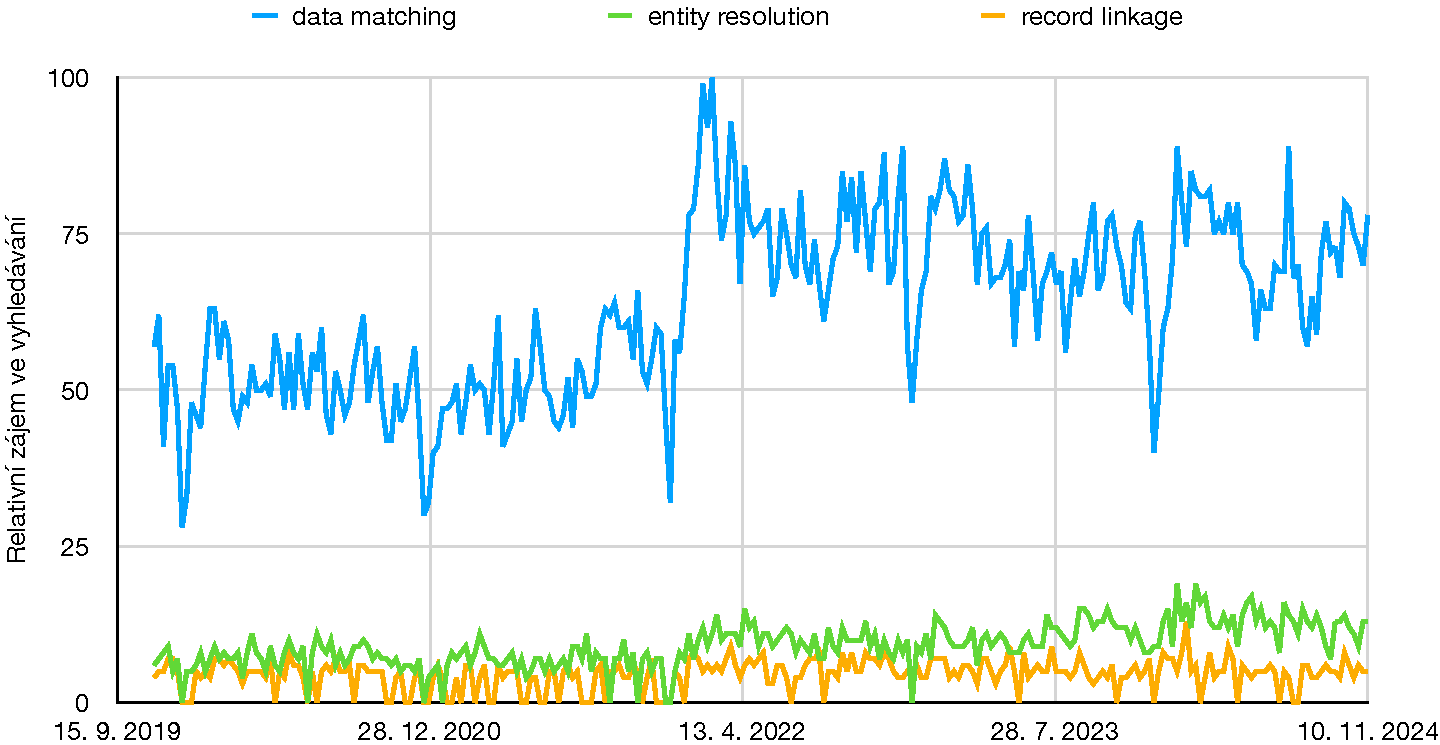
\includegraphics[scale=0.6]{images/google-trends.pdf}
  \caption{Zájem o termíny "data matching", "entity resolution" a "record linkage".\newline
    \textit{Zdroj}: \cite{google_trends_google_2024}}
  \label{fig:google-trends}
\end{figure}
\pagebreak

\sekce{Příčiny vzniku duplicit}
Zazněli zde již některé důvody vzniku duplicit v datech, pojdmě se blíže podívat na nejčastější z nich. Rozdělil jsem je zde na duplicity v datech, které mohou vzniknout v rámci jednoho datového zdroje, a duplicity vznikající spojením více datových zdrojů.

\podsekce{Duplicity v samostatném zdroji}
Přestože by se na první pohled zdálo, že v rámci jednoho datového zdroje šance na vznik duplicity minimiální, je zde i tak několik případů, které vedou ke vzniku duplicit. Tady jsou některé z nich:

\begin{itemize}
  \item Lidský faktor – při zadávání dat člověkem ručně je velká pravděpodobnost zadání typografických chyb, různých nekonzistentních formátů a nebo přímo neplatných informací. Při zadávání dalších záznamů si pak daný člověk nemusí všimnout již existujícího záznamu vloženého dříve.
  \item Nedostatečné standardizace formátů – různé formuláře, dotazníky, nebo části/moduly jednoho systému mohou využívat různé formáty pro datumy, telefonní čísla, nebo rodná čísla a dalších typů dat. Pokud není správně ošetřen převod těchto dat do jednotného formátu před vložením záznamu, může opět docházet ke vzniku duplicit.
  \item Chybějící integritní omezení databáze – kdyby byly sebevíce ošetřeny předchozí zmíněné způsoby, v případě, že daná databáze nemá nastavená integritní omezení (např. na unikátní hodnoty v rámci rodného čísla, IČO nebo třeba unikátnosti dvou a více atributů v rámci jednoho záznamu), bude každý vložený záznam brán jako nový neexistující záznam, přestože se bude jednat o identickou duplicitu.
\end{itemize}

\podsekce{Duplicity ve sloučeném zdroji}
Při pokusu o spojení více zdrojů do jednoho vzniká několik výzev. V rámci business inteligence se tento proces nazývá ETL\footnote{Extract, transform, load
} v rámci něj může docházet k duplicitám v několika případech:

\begin{itemize}
  \item Integrace různých systémů – v případě systémů, které mají data o entitách kvůli různým důvodům (např. inventární systém školy ukládá záznamy o vybavení, online bazar má záznamy o prodávaném vybavení), může vzniknout situace, kdy záznamy z více systémů nelze spojit na základě společného unikátního klíče, protože má každý systém svůj unikátní pro danou entitu.
  \item Průběžné spojování dat – některé datasety jsou pravidelně aktualizované, aby odráželi co nejvíce realitu. Pokud však entita z realného světa v rámci aktuality změnila zásadně své atributy (např. pekárna se přestěhovala na jinou adresu a přejmenovala se), může vzniknout situace, kdy některý ze zdrojů bude mít stále staré údaje, a jiný nové, a tím pádem nepůjde tento rozdíl spojit s původním záznamem a bude se milně jevit, že jde o novou entitu
  \item Ještě jeden...
\end{itemize}




\podsekce{Dopady duplicit na analýzu a rozhodování}

% Příkladem kdy k takovému problému nedojde může být případ z prostředí České republiky a předpokládejme, že jde o data čistě občanů České republiky, kdy máme první datový zdroj s pacienty ordinace a druhý zdroj je databáze klientů zdravotní pojišťovny. V tomto případě lze snadno rozpoznat dané entity (osoby) na základě rodného čísla, které se u záznamů v těcho zdrojích pravděpodobně nachází. V tomto případě můžeme následně data zagregovat a dále s nimi pracovat.

\sekce {Přístupy k~rozpoznání duplicitních entit}
Detekce duplicit bez využití strojového učení zahrnuje například algoritmus pro výběr párů Sorted-Neighborhood-Method (SNM). Je možné provést porovnání všech možných kombinací záznamů, ale SNM efektivně snižuje počet nutných porovnání tím, že seřadí data a porovnává pouze sousední záznamy. Pro následné měření podobnosti mezi záznamy se často používají metody jako Jaro-Winkler a Levenshtein, které posuzují, do jaké míry se záznamy podobají. Na základě takové podobnosti lze určit, zda jsou porovnané záznamy duplicity. Tyto metody jsou obzvláště užitečné pro identifikaci menších rozdílů a překlepů ve zpracovávaných datech. \cite{draisbach_choosing_2013}

Metody strojového učení nabízí pokročilejší možnosti, které umožňují identifikovat složitější vzory, které by metody bez využití strojového učení nemuseli odhalit. Například, hluboké neuronové sítě mohou být trénovány na rozsáhlých datových sadách a díky tomu mohou nalézt v datech složité vzory. Takto natrénované neuronové sítě mohou označit za duplicitní záznamy, které na první pohled jako duplicity nevypadají. \cite{pasek_mqdd_2022}
% \todo{Algoritmy a techniky}

\sekce {Specifika geoprostorových dat}
% \todo {Typy geodat(vector, body, linie a rastry), formáty uložení, souřadnicové systémy}
Jde o~data, která představují místa, oblasti nebo třeba předměty ze skutečného světa, a udávají jejich přesnou lokalitu pomocí souřadnic na Zemi. Můžeme mít například geodata představující státní hranice evropských zemí, geodata představující všechny lampy veřejného osvětlení v~Brně.
% \todo{Obrázek s~GIS mapama}

\podsekce{Souřadnicové systémy}

Geodata používají souřadnice pro popsání pozice konkrétního objektu. Těchto souřadnic však existuje hned několik a při práci s~geodaty je potřeba vědět, které to jsou. Existují různé typy souřadnicových systémů, které se používají podle konkrétních požadavků. Mezi nejpoužívanější v~kontextu České republiky patří:

\podsekce{Globální a celosvětové použití}

\podsekce{Geografický souřadnicový systém (GCS) - WGS 84}

Systém využívající úhlových souřadnic, konkrétně zeměpisné šířky a délky. Nadmořská výška se udává v~metrech nad povrchem referenčního elipsoidu.
Je vhodný pro geodata představující entity na celosvětové úrovni. Díky tomu je využíván například i v~GPS technologii, kde je zapotřebí pracovat v~rámci celé Země.
Není však příliš vhodná pro lokální úroveň (města, ulice), pokud je vyžadována vysoká přesnost. Je tomu tak protože při výpočtu vzdáleností nebo ploch z~úhlových souřadnic může docházet k~nepřesnostem.

\podsekce{Regionální a národní použití}

\podsekce{Projekční souřadnicový systém (PCS) - S-JTSK (Systém Jednotné Trigonometrické Sítě Katastrální)}

Tento konkrétní systém je navržen pro Českou republiku a umožňuje tak na jejím území mapovat s~vysokou přesností. Je proto používán jako jeden ze závazných souřadnicových systémů pro orgány České republiky.
Souřadnice jsou vyjádřeny pomocí kartézského souřadnicového systému (X - sever, Y - východ) a jednotkou jsou metry. Pro nadmořskou výšku používá metry nad střední hladinou Jaderského moře.

\podsekce{Evropský souřadnicový systém - ETRS89 (European Terrestrial Reference System 1989)}

Souřadnicový systém ETRS89 slouží jako standard pro evropské projekty a díky tomu i usnadňuje spolupráci vícero zemí na projektech s~mezihraničním rozsahem.
Stejně jako S-JTSK používá kartézský souřadnicový systém v~jednotkách metru. Výška v~tomto systému je počítáná v~metrech od povrchu referenčního elipsoidu GRS80.

Toto nejsou zdaleka všechny souřadnicové systémy. Každý z~nich slouží pro jiné potřeby a je důležité si uvědomit, jak se liší, a v~jakém kontextu se s~nimi lze setkat.

% \todo{Tvary geodat (points, lines, and polygons)}

\podsekce{K~čemu slouží}

Geodata sama o~sobě ale popisují vždy specifický objekt. Aby se dali z~těchto dat získat nějaké znalosti, je potřeba je dále zpracovávat. K~tomu slouží například geografické informační systémy (GIS). Tyto systémy dokáží poskytnutá data analyzovat a vizualizovat a dále s~nimi pracovat dle potřeby. Mohou tak umožnit například přehledně vidět, v~jakém úseku silnice je v~daný čas nejvíce aut, a zároveň vidět, ze kterých navazujících silnic tam tyto auto přijíždí. Díky takové vizualizaci a analýze lze následně vycházet například při plánování dopravní infrastruktury.

Každý kdo otevře služby jako Google Maps, Seznam Mapy nebo Apple Maps se dívá na několika vrstvou vizualizaci geodat. Na první pohled se jedná o~běžnou mapu, avšak vizualizace v~těchto službách je běžně tvořena několika samostatnými vrstvami:

\begin{itemize}
  \item vrstvy komunikace,
  \item vrstvy staveb,
  \item vrstvy řek,
  \item vrstvy zeleně a dalších.
\end{itemize}

% \todo{Obrázek map z~aplikací}
Každá taková vrstva je sada geodat, která popisuje daný typ předmětu/lokace s~přesnými souřadnicemi dalšími pomocnými atributy/vlastnostmi.

\sekce {Existující nástroje}
% \todo{Popište dostupné software, jejich výhody a nevýhody}
